\chapter{Design Choices}


\section{Where should electronic complexity lie?}
\label{sec:complexity}

Some form of electronic device has to be used to identify the relative positions of the rods, but we have some choice in where this device exists. If we want to keep our product to be simply a set of rods, then the only place for the device is within the rods themselves. The rods would each need to be able to communicate with each other, to discern relative position, and also with either a controller that relays messages to the server or to the server directly.\\

Unfortunately, this solution brings several impracticalities. Firstly, the size of the rods has to be kept small, which constrains the size of battery we could embed into them. They will have to be capable of transmitting and receiving wireless messages, and even perhaps perform some amount of processing, so their power consumption will be too high for a battery of that size. Charging the batteries would also be impracticable; consider a classroom of around 30 students, each with a set of dozens of rods, and it becomes clear that the hassle of having to charge each device individually would outweigh any benefit of the product to a teacher.\\

Another issue concerns the identification of rods and their assignment to students: remember again that each student needs their own set of dozens of rods, and that any information these rods transmit will be attached to that child’s profile. The teacher would have to perform the frustrating and repetitive task of assigning each rod to a student, causing a considerable amount of inconvenience. Additionally, we must keep in mind that our target users are children, who may have the tendency to take rods from another student, misplace their own rods, or perhaps even throw rods around the classroom – all of these actions could cause sets of rods to be mixed together, leading to incorrect data being sent to the server, as progress from one student will be attached to the profile of another.\\

The last issue is economic: each of these rods will require several electronic components, including a processing unit and wireless transceivers, driving the cost of each unit up considerably. This is especially relevant as the smaller rods are easily lost in the classroom, so replacements would likely need to be purchased, increasing ongoing costs further.\\

An alternative solution to putting complexity in the rods is to design a playing board with which the rods can interact, and embed the majority of the electronics in that instead. The 10x10 board would resemble a chess board, with grid squares guiding the placement of rods. The students arrange their rods on the board, which can identify the positions of the rods through some means, and communicate that data to the server. This alleviates all of the problems detailed above. The board is large and can house a larger battery than the rods, so there would be no power problem. There would only be one board per child so there are fewer devices to charge and much less work involved in assigning devices to children, also meaning that mixing of rods is not an issue, as it is the board which is unique to the child, not the rods. The cost to replace rods would be much lower as they would not contain as much electronics, and the overall cost would be lower as only the boards would require processing and communications equipment, as opposed to fitting one to every rod.\\ 

During an interview with a primary school teacher, we were informed that having a board may actually aid in the students’ learning, as having a grid could help them conceptualise how the rods fit together. 

\section{How should the board detect rod positions?}
\label{sec:detection}  


Having settled on the use of a board, the next design choice to be made is what technology it will make use of to detect where rods have been placed. The chosen method needs to have the following characteristics to be viable: it must be able to \textit{reliably} detect rods and their positions, as any errors may mislead and confuse the child, weakening the product’s effectiveness as an educational tool. It should keep \textit{cost} low, as there could be up to hundreds of these products in use at an institution, and since they will likely be using public funding they will be under budget constraints. It should keep \textit{power consumption} to a minimum to maximise the amount of use between charges. Lastly, it should remove as much \textit{complexity} from the rods as possible, for the reasons outlined in section \ref{sec:complexity}.\\

%%  Weight %%

\subsection{Weight}
\label{weight}

Rods could be given different weights, which are sensed by load sensors on the board. Each weight would be mapped to a different length of rod.\\

{
\setlength{\parindent}{0pt} % Remove paragraph indents within this block

\textbf{\textit{Reliability:}} It may be difficult to distinguish between the weight of a rod and the weight from the child touching the board, which could lead to false readings. However, under good conditions it should be possible to distinguish between rods well.\\

\textbf{\textit{Cost:}} The cost of the rods will likely be low, as they will just require weighting, however the board will require a load sensor in every grid square. The load sensor would need to be small enough to fit into a square around $2cm^2$ in area, and be sensitive enough to detect weighted rods light enough for a child to safely play with. A preliminary search revealed that components meeting those specifications would cost tens of pounds  \cite{ref:loadsensor}. Considering we are using a 10x10 board, purchasing 100 of these components would increase the cost to unacceptable levels.    \\

\textbf{\textit{Power Consumption:}} The datasheet of a suitable sensor \cite{MICROSWI18:online} states a typical voltage requirement of $10V$, and an input resistance of $5k\Omega$. Using $P=\frac{V^2}{R}$ we can determine a power usage of $0.02W$. 100 of these components would then draw 2W, which is relatively high, but could be acceptable depending on the battery used. \\

\textbf{\textit{Rod Complexity:}} The rods will not need any electronics, just some weighted material, so the complexity is quite low.\\
}

%%  Magnets %%

\subsection{Magnetic Fields}
\label{magnets}

Magnets of varying strength could be inserted into rods to be detected by gaussmeters in the board. Each strength would be mapped to a different length of rod. \\

{
\setlength{\parindent}{0pt} 

\textbf{\textit{Reliability:}} In theory, a system using magnets could be quite reliable, as rare earth magnets can be used for several years without their strength diminishing \cite{Permanen88:online}.    \\

\textbf{\textit{Cost:}}\\

\textbf{\textit{Power Consumption:}}\\

\textbf{\textit{Rod Complexity:}} The rods would be kept quite simple, as they would just require a magnet inserted into them.\\
}

%%  RFID %%

\subsection{RFID}
\label{rfid}

Passive RFID chips could be inserted into the rods, and RFID sensors into the board. Each RFID chip would contain identifying information about the rod it is in. When a rod is placed on the board, its RFID chip is powered and the data is read, and sent to the server. \\

{
\setlength{\parindent}{0pt} 

\textbf{\textit{Reliability:}} Our requirements are such that the range of detection of a rod should be very small, no more than a centimetre or so, as otherwise neighbouring grid squares could erroneously detect nearby rods and send false data to the server. A search for RFID products that operate in this range found no suitable results, which indicates RFID is not tailored to the precision detection needed for this project.\\

\textbf{\textit{Cost:}} An example of one of the shortest range components of the correct dimensions retails at between £5-14 per unit \cite{RITRPR9U23:online}; while this is much cheaper than the load sensor described above, it would still raise the price of the product to an unacceptable level given the quantity of boards/rods needed for a classroom.\\

\textbf{\textit{Power Consumption:}} Since the components in the rod are passive, they would draw a minimal amount of power \\

\textbf{\textit{Rod Complexity:}} Since this solution requires inserting electronics into the rods, the complexity is quite high. This increases the chance that something may fail and rods will need to be replaced. Another problem is that readings will be inaccurate until the fault is discovered, which may take some time. \\
}


%%  RGB %%

\subsection{RGB Light}
\label{rgb}

Each grid square of the board could contain an RGB LED and a photodiode; the LED would flash periodically and the photodiode would measure the frequency of the reflected light. Since each rod is of a distinctly different colour, each would produce a different reflected frequency.\\

{
\setlength{\parindent}{0pt} 

\textbf{\textit{Reliability:}} This method has the potential for very good reliability, as there are few enough different sizes of rod such that each can have a distinct colour, which reduces the possibility of a false reading. However, it is unclear how such a system might respond to a different object like a child's hand being placed on the board. \\

\textbf{\textit{Cost:}} The cost of the components for this design is quite high: 100 pairs of a suitable photodiode \cite{KPS5130P52:online} and LED \cite{L154A4SU86:online} would cost over £150.  \\

\textbf{\textit{Power Consumption:}} \\

\textbf{\textit{Rod Complexity:}} This method requires adding nothing at all to the rods: since the solution works by sensing colour, the rods would be just plain coloured plastic.\\
}

%%  Resistors %%

\subsection{Shorting Resistor Chains}
\label{resistors}

Each row on the board could be linked by a long series chain of resistors of known values, and the rods themselves could contain a wire connecting two contacts, on either end of the rod. Each row would have its own chain, connected in parallel to the other chains. When the rod is placed on the board, its contacts would connect to contacts on the board, shorting a number of resistors in the board relative to the rod's length. The change in voltage at the different nodes in the line could be used to detect if and where a rod is placed.\\

{
\setlength{\parindent}{0pt} 

\textbf{\textit{Reliability:}} This solution will be very reliable as long as the contacts are designed in such a way that a child could not short resistors without a rod, which would produce a false reading. Another requirement is that the voltage level be high enough so that every node in the chain of resistors is sufficiently different and distinguishable.\\

\textbf{\textit{Cost:}} The only component required is resistors, which are much cheaper \cite{CFR25J1024:online} than the resources required for the alternative solutions.\\

\textbf{\textit{Power Consumption:}} The power consumption will be low: assuming the board will be controlled by a microcontroller with a 5V rail powering 10 parallel chains of resistors each totalling $2K\Omega$ (meaning the overall resistance is $200\Omega$), a $P=\frac{V^2}{R}$ calculation reveals a power usage of $0.125W$, which is quite acceptable.  \\

\textbf{\textit{Rod Complexity:}} The rods will be kept relatively simple, as they will just need a wire between the two contacts inside them, however the design of the contact could increase complexity.\\
}




Considering the above comparison, the best solution is the resistor chains; it is comparatively inexpensive, uses comparatively low power, and does not rely on any complex technologies so has high reliability. The complexity of the rods is slightly increased due to the need for contacts, but faults with these should be more apparent than faults with electronics embedded in a rod, and in the event of a fault, replacement rods will not incur significant cost.

%%				%%
%%  Prototyping	%%
%%				%%

\section{Prototyping}

\subsection{Controller}
To control the reading of data from the resistor chains, it was decided to make use of an Arduino microcontroller board \cite{ArduinoH73:online}. This was mainly because of its ease of use, and active community of users who can provide support during the prototyping process. The Arduino board provides an interface to external hardware via GPIO pins that can be used to read the voltages along the chain of resistors, and has a 5V power rail that can be used to power the prototype. 

\subsection{Mapping Voltage Values to Rod Placement}
\label{sec:voltages}
Prototyping began with the construction of two parallel simple resistor chains (shown in Figure \ref{fig:simple_resistor}) to learn to use the Arduino and to get some intuition on how rod placement could be ascertained from the measured voltages. 

\begin{figure}[H]
	\begin{center}
	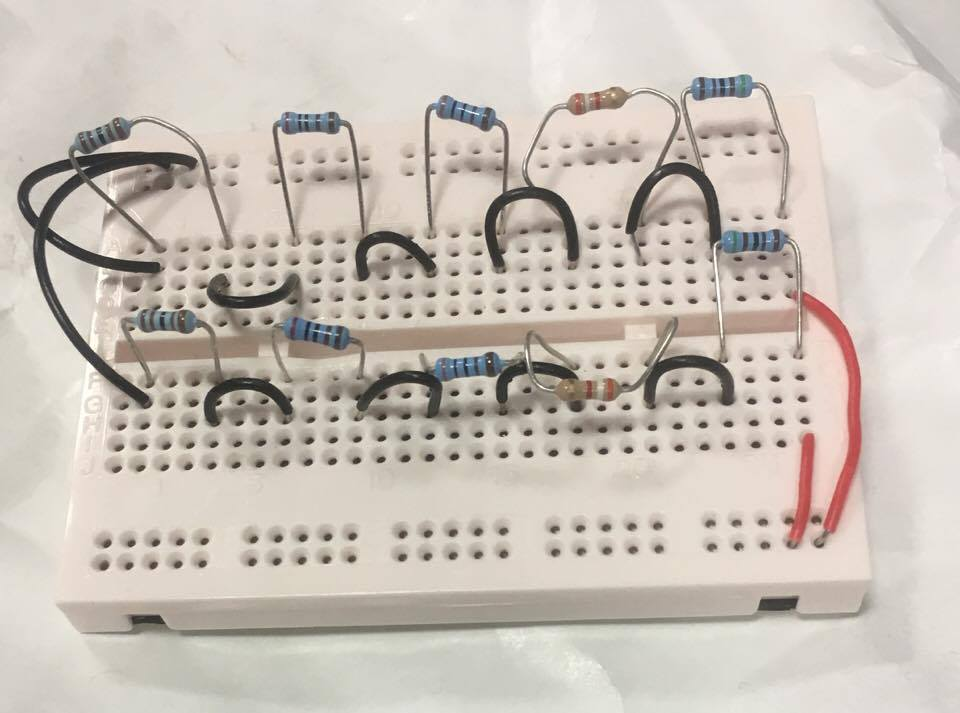
\includegraphics[width=0.75\textwidth]{simple_resistor_chain.jpg}\\
  	\caption{Parallel Resistor Chains}
    \label{fig:simple_resistor}
    \end{center}
\end{figure}

This first attempt incorporated the use of differing resistors down the chain, as in Figure \ref{fig:simple_resistor} (although it was later realised that using equal resistors would be better suited as they would give uniform increments of voltage at each node along the chain). A wire was used to connect two of the labelled nodes A-E to represent the functionality of the rod shorting resistors. Voltage was measured at two points along the chain (Figure \ref{fig:5r}) to see if each different position of the rod along a chain could produce a unique pair of voltages that could be used to identify that position.  \\



\begin{figure}[H]
	\begin{center}
	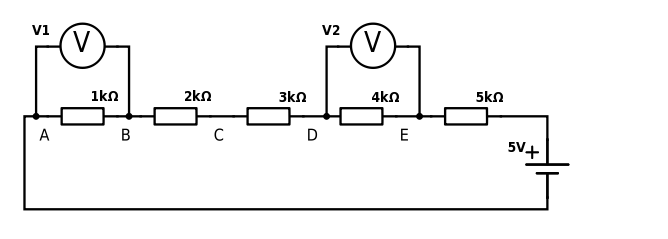
\includegraphics[width=0.8\textwidth]{5r.png}\\ 
  	\caption{Simple prototype with labelled nodes}
    \label{fig:5r}
    \end{center}
\end{figure}



\begin{table}[H]
\centering
\begin{tabular}{c|ccccc}
\cline{2-6}
                                 & \multicolumn{1}{c|}{\textbf{A}}                 & \multicolumn{1}{c|}{\textbf{B}}                 & \multicolumn{1}{c|}{\textbf{C}}                 & \multicolumn{1}{c|}{\textbf{D}}                 & \multicolumn{1}{c|}{\textbf{E}}                 \\ \hline
\multicolumn{1}{|c|}{\textbf{A}} & \multicolumn{1}{c|}{\cellcolor[HTML]{C0C0C0}}   & \multicolumn{1}{c|}{0, 3.18}                    & \multicolumn{1}{c|}{0, 2.88}                    & \multicolumn{1}{c|}{0, 2.17}                    & \multicolumn{1}{c|}{0, 0}                       \\ \cline{1-1} \cline{3-6} 
\multicolumn{1}{|c|}{\textbf{B}} & \cellcolor[HTML]{C0C0C0}                        & \multicolumn{1}{c|}{\cellcolor[HTML]{C0C0C0}}   & \multicolumn{1}{c|}{0.41, 3.05}                 & \multicolumn{1}{c|}{0.53, 2.47}                 & \multicolumn{1}{c|}{0.87, 0.87}                 \\ \cline{1-1} \cline{4-6} 
\multicolumn{1}{|c|}{\textbf{C}} & \cellcolor[HTML]{C0C0C0}                        & \cellcolor[HTML]{C0C0C0}                        & \multicolumn{1}{c|}{\cellcolor[HTML]{C0C0C0}}   & \multicolumn{1}{c|}{0.44, 2.89}                 & \multicolumn{1}{c|}{0.66, 1.89}                 \\ \cline{1-1} \cline{5-6} 
\multicolumn{1}{|c|}{\textbf{D}} & \cellcolor[HTML]{C0C0C0}                        & \cellcolor[HTML]{C0C0C0}                        & \cellcolor[HTML]{C0C0C0}                        & \multicolumn{1}{c|}{\cellcolor[HTML]{C0C0C0}}   & \multicolumn{1}{c|}{0.48, 2.73}                 \\ \cline{1-1} \cline{6-6} 
\multicolumn{1}{|c|}{\textbf{E}} & \cellcolor[HTML]{C0C0C0}{\color[HTML]{333333} } & \cellcolor[HTML]{C0C0C0}{\color[HTML]{333333} } & \cellcolor[HTML]{C0C0C0}{\color[HTML]{333333} } & \cellcolor[HTML]{C0C0C0}{\color[HTML]{333333} } & \cellcolor[HTML]{C0C0C0}{\color[HTML]{333333} } \\ \cline{1-1}
\end{tabular}
\caption{Voltages (V1, V2) when two nodes are connected by a wire}
\label{tab:5r_voltages}
\end{table}

The values in Table \ref{tab:5r_voltages} show the voltages at V1 and V2 when each pair of nodes is connected. It is apparent that every combination of connected nodes does produce a unique pair of voltages, which proves that it is possible, in principle, to identify rods based on the voltages of the nodes. This experiment was a proof-of-concept, as it only used 5 resistors, but the real prototype needs at least 10 resistors to detect rods of up to size 10.

\subsection{The Problem with the Unit Rod}

At the end of Section \ref{sec:voltages} we postured that we would need at least 10 resistors per chain to detect rods of up to size 10; while this is true, it overlooks the necessity to detect unit rods, of size 1. The assumption is that each node in the resistor chain is connected to a grid square on the board, and that rods spanning multiple grid squares can short the resistors between those two nodes when connected to the board. However, a unit rod spans only one grid square, meaning that it is only connected to one node, and so cannot short any resistors. Figure \ref{fig:unitrod} demonstrates why this is the case. Note that the representations of the wires connecting the rods and the resistor chain are symbolic and do not represent what the actual connections would look like.

\begin{figure}[H]
	\begin{center}
	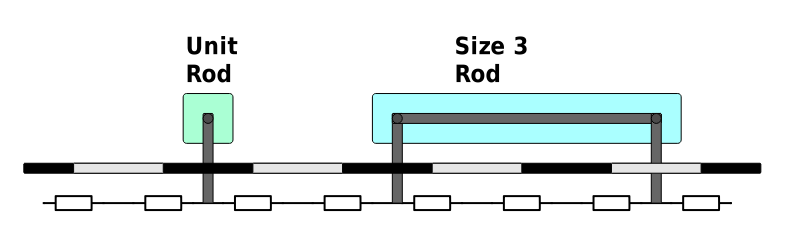
\includegraphics[width=0.8\textwidth]{unitrod.png}\\ 
  	\caption{Cross-sectional view of board}
    \label{fig:unitrod}
    \end{center}
\end{figure}

The chosen solution to this problem was add a double connector to the unit rod instead of the unit one, so that it can connect to two nodes and short a resistor. This means that twice as many resistors are required along a chain, but allows us to detect unit rods without affecting the detection of the other sizes.

\begin{figure}[H]
	\begin{center}
	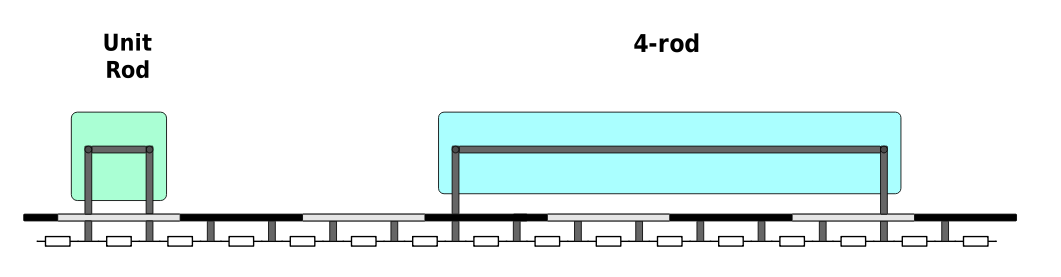
\includegraphics[width=\textwidth]{doubleunitrod.png}\\ 
  	\caption{Cross-sectional view of board with double resistor chain length}
    \label{fig:doibleunitrod}
    \end{center}
\end{figure}

%Two-value measurement table\\ 
%Why it wasnt suitable, needed to measure every node instead

\subsection{Practicalities in Data Measurement}
%Multiplexers: why you need them instead of 2-value measurement


